\documentclass[a4paper, 12pt]{article}

\usepackage[portuges]{babel}
\usepackage[utf8]{inputenc}
\usepackage{amsmath}
\usepackage{indentfirst}
\usepackage{graphicx}
\usepackage{multicol,lipsum}
\usepackage{hyperref}
\usepackage{minted}

\begin{document}
%\maketitle

\begin{titlepage}
	\begin{center}
	
	%\begin{figure}[!ht]
	%\centering
	%\includegraphics[width=2cm]{c:/ufba.jpg}
	%\end{figure}

		\Huge{Instituto de Ciências Matemáticas e de Computação}\\
		\large{Departamento de Ciências de Computação}\\ 
		\large{SCC0503 - Algoritmos e Estruturas de Dados II}\\ 
		\vspace{15pt}
        \vspace{95pt}
        \textbf{\LARGE{Relatório Exercício 04}}\\
		%\title{{\large{Título}}}
		\vspace{3,5cm}
	\end{center}
	
	\begin{flushleft}
		\begin{tabbing}
			Alunos: Ryan Souza Sá Teles, Silmar Pereira da Silva Junior \\
            NUSP's: 12822062, 12623950.
			Professor: Leonardo Tórtoro Pereira\\
			%Professor co-orientador: \\
	\end{tabbing}
 \end{flushleft}
	\vspace{1cm}
	
	\begin{center}
		\vspace{\fill}
			 Junho\\
		 2022
			\end{center}
\end{titlepage}
%%%%%%%%%%%%%%%%%%%%%%%%%%%%%%%%%%%%%%%%%%%%%%%%%%%%%%%%%%%

\newpage
% % % % % % % % % % % % % % % % % % % % % % % % % %
\newpage
\tableofcontents
\thispagestyle{empty}

\newpage
\pagenumbering{arabic}
% % % % % % % % % % % % % % % % % % % % % % % % % % %
\section{Introdução}
O exercício consiste na leitura de dados de quests (missões) de um jogo e na construção de um dígrafo com estes dados e a simulação da execução delas através da travessia em profundidade do dígrafo.
\newpage
\section{Desenvolvimento}

O desenvolvimento do projeto fez uso das abstrações já adotadas em sala de aula e o modelo de dígrafo selecionado para trabalhar foi o de "lista de adjâcencias", o porque desta escolha deve-se ao fato de que [Justificar o motivo].

Com o objetivo de aplicar as boas práticas de código na atividade, foi criado a classe "Answer" que se tornou classe mãe da Vertex, a qual, possui o método "toString" que imprime na tela cada vertice.

Implementação da classe Answer:

\begin{minted}[mathescape, linenos]{java}

public class Answer {
    private int id;
    private String name;
    private String description;
    
    public Answer(int id, String name, String description) {
        this.id = id;
        this.name = name;
        this.description = description;
    }
    
    public int getId() {return id;}
    public String getName() {return name;}
    public String getDescription() {return description;}
    public void setId(int id) {this.id = id;}
    public void setName(String name) {this.name = name;}
    
    public void setDescription(String description) {
        this.description = description;
    }
    public String toString() {
        return "Quest{\n\tID: " + id + "\n\tName: " + name + "\n\tDescription: " + description + "\n}";
    }
}


\end{minted}


Para a implementação do algoritmo de busca em profundidade, por questões didáticas e não de desempenho algorítmico, foi criado o método "getAllConnectedVertex" dentro da classe "DigraphList" e definido seu contrato na interface "GraphInterface", abaixo a implementação:
\begin{figure}[h!]
\center 
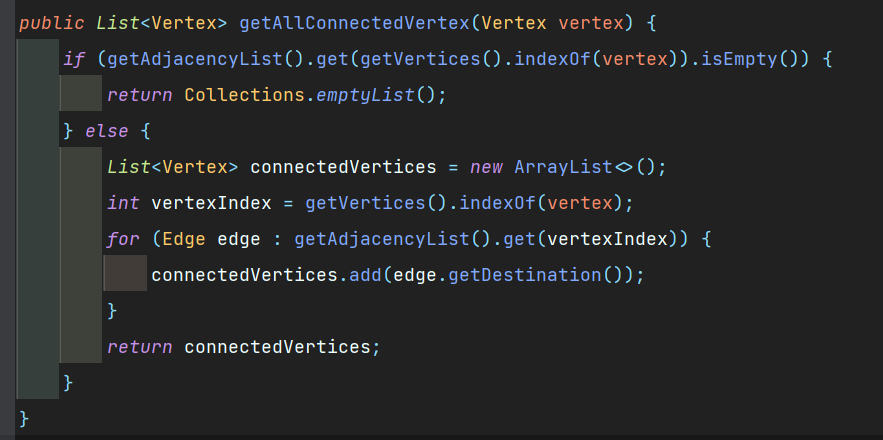
\includegraphics[width=.8\textwidth]{getAllConnectedVertexMethod.png}
\caption{Implementação do método getAllConnectedVertex}
\end{figure}

A implementação do algoritmo Depth First Search: 
\begin{figure}[h!]
\center 
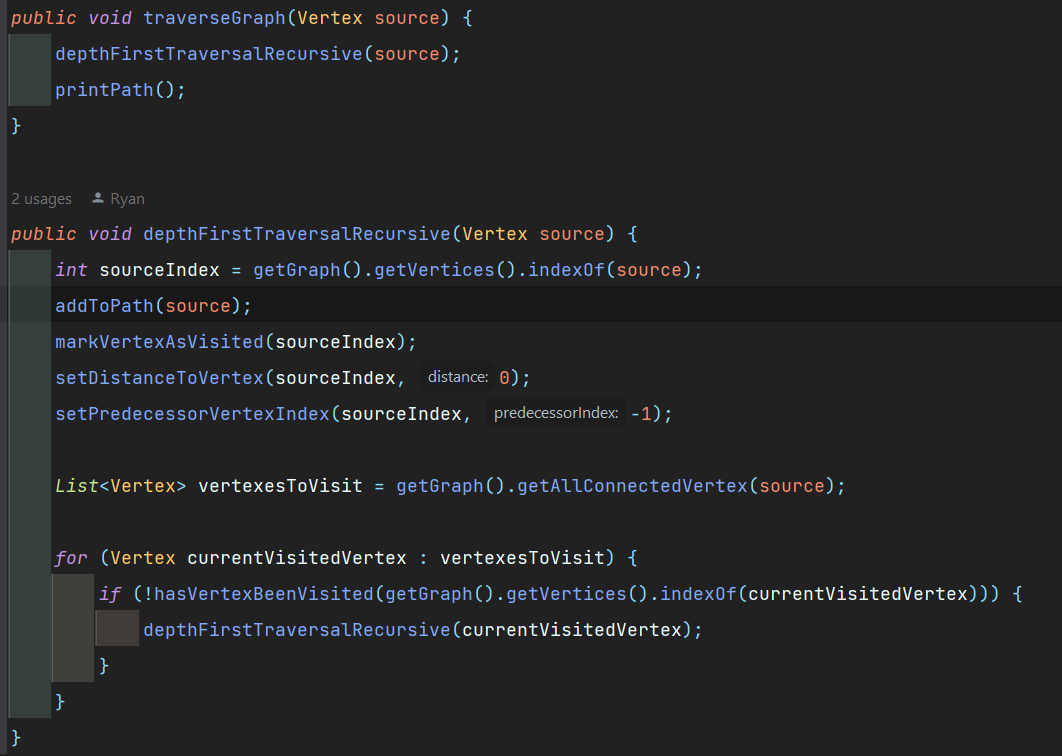
\includegraphics[width=.8\textwidth]{depthFirstTraversalRecursiveMethod.png}
\caption{Implementação do algoritmo Depth First Search}
\end{figure}

Como modelo de busca recursiva para o algoritmo, ele sempre vai estar indo do primeiro vertice adicionado como aresta a partir do vertice de origem.

Descreva os principais pontos do desenvolvimento do projeto. Algoritmos utilizados, decisões de projeto que sejam relevantes, etc.
Se ajudar no entendimento, coloque pseudo-códigos ou prints de código de áreas importantes.

Se precisar citar algo, adicione a formatação em bibtex no arquivo \textit{bibliography.bib} e cite com o comando \textit{\textbackslash cite}, assim: \cite{even2011graph}

Para imagens, pode começar uma \textit{figure} e chamar o comando \textit{\textbackslash includegraphics}, assim:

\begin{figure}[h!]
\center 

\includegraphics[width=.8\textwidth]{logo.png}
\caption{Logo do ICMC com uma legenda}
\end{figure}

Para tabelas, recomendo criar e exportar deste cite aqui (alias, é assim que adiciona URL -  \textit{\textbackslash url}): \url{https://www.tablesgenerator.com/}

\newpage
\section{Resultados}
Prints do grafo juntamente com sua saída:


Aqui, coloque imagens/tabelas/textos com os resultados, discuta brevemente o que foi obtido.
\newpage
\bibliographystyle{plain}
\bibliography{bibliography.bib}
\newpage
\addcontentsline{toc}{section}{Anexo}
\section*{Anexo}
No anexo, pode colocar qualquer coisa extra que achar interessante: detalhes mais completos de resultados, alguma coisa diferente/inovadora que fez, etc.
\end{document}



